\documentclass[12pt]{article}

\usepackage{graphicx}% Include figure files
\usepackage{dcolumn}% Align table columns on decimal point

% Use Arial font %
\usepackage{helvet}
\renewcommand{\familydefault}{\sfdefault} 

% Default margins and paper properties %
\usepackage[a4, portrait, margin=0.6in]{geometry}

\begin{document}
	\title{Hypothesis plots summary} % Force line breaks with \\
	\author{1666957, Gustavo Espinal Lugo}
	\date{\today} % It is always \today, today, %  but any date may be explicitly specified

	\maketitle
	%\tableofcontents
	
	\section*{Plots and corresponding metadata}
	Number of data points used: 99999,\\
mean expected W mass: 80.36010913 $[GeV/c^{2}]$,\\
mean hypothesis masses $[GeV/c^{2}]$: [<generator object <genexpr> at 0x7f820a339510>],\\
mass width: 2.07041274 $[GeV/c^{2}]$,\\
chi\_square value of hypothesis fit: 112.07408778430181\\
	Absolute path to figure: /home/physics/phuxdp/Desktop/PX402 Physics Project/WBosonProject/noQED/plots/muPT\_80.36010913\_2.07041274\_between\_71\_and\_91.png\\
	Next lines are the data of the shown histograms (if needed): \\
	All quantities: 	99999, 80.36010913, [71. 73. 75. 77. 79. 81. 83. 85. 87. 89. 91.], 2.07041274, 112.07408778430181\\
	X\_energ\_vls = [30.1, 30.299999999999997, 30.5, 30.700000000000003, 30.9, 31.1, 31.299999999999997, 31.5, 31.700000000000003, 31.9, 32.1, 32.3, 32.5, 32.7, 32.9, 33.1, 33.3, 33.5, 33.7, 33.9, 34.1, 34.3, 34.5, 34.7, 34.9, 35.1, 35.3, 35.5, 35.7, 35.9, 36.1, 36.3, 36.5, 36.7, 36.9, 37.1, 37.3, 37.5, 37.7, 37.9, 38.1, 38.3, 38.5, 38.7, 38.9, 39.1, 39.3, 39.5, 39.7, 39.9, 40.1, 40.3, 40.5, 40.7, 40.9, 41.1, 41.3, 41.5, 41.7, 41.9, 42.1, 42.3, 42.5, 42.7, 42.9, 43.1, 43.3, 43.5, 43.7, 43.9, 44.1, 44.3, 44.5, 44.7, 44.9, 45.1, 45.3, 45.5, 45.7, 45.9, 46.1, 46.300000000000004, 46.5, 46.7, 46.9, 47.1, 47.300000000000004, 47.5, 47.7, 47.9, 48.1, 48.300000000000004, 48.5, 48.7, 48.9, 49.1, 49.300000000000004, 49.5, 49.7, 49.9]\\
	Y\_data\_bin\_cnts = [266.0, 281.0, 301.0, 304.0, 281.0, 321.0, 336.0, 324.0, 300.0, 328.0, 328.0, 325.0, 318.0, 337.0, 328.0, 371.0, 345.0, 331.0, 383.0, 356.0, 327.0, 345.0, 368.0, 354.0, 369.0, 369.0, 367.0, 344.0, 389.0, 342.0, 384.0, 374.0, 371.0, 385.0, 365.0, 370.0, 364.0, 348.0, 351.0, 340.0, 420.0, 408.0, 389.0, 399.0, 403.0, 398.0, 377.0, 376.0, 348.0, 319.0, 320.0, 307.0, 319.0, 305.0, 286.0, 320.0, 272.0, 260.0, 239.0, 235.0, 228.0, 215.0, 216.0, 211.0, 204.0, 180.0, 196.0, 185.0, 158.0, 154.0, 148.0, 127.0, 134.0, 128.0, 120.0, 120.0, 123.0, 101.0, 104.0, 94.0, 110.0, 105.0, 81.0, 79.0, 100.0, 86.0, 75.0, 76.0, 86.0, 83.0, 80.0, 77.0, 65.0, 70.0, 73.0, 61.0, 64.0, 56.0, 57.0, 66.0]\\
	Y\_model\_bin\_cnts = [248.8841552734375, 201.95858764648438, 216.60215759277344, 280.37548828125, 141.84603881835938, 104.4836196899414, 249.8253631591797, 32.915679931640625, 152.64610290527344, 239.68687438964844, 58.53604507446289, 106.0986099243164, 170.5635528564453, 409.2520751953125, 259.4189758300781, 144.86660766601562, 47.69832229614258, 179.67138671875, 73.05419921875, 299.77728271484375, 83.81353759765625, 252.1007080078125, 196.16159057617188, 353.58428955078125, 142.7912139892578, 178.62359619140625, 453.01873779296875, 377.9122314453125, 94.9889144897461, 82.77993774414062, 115.96817016601562, 345.4283752441406, 138.16693115234375, 557.5431518554688, 103.93212127685547, 258.90179443359375, 162.27090454101562, 409.20709228515625, 205.798583984375, 174.62045288085938, 75.85962677001953, 195.6945343017578, 218.5081329345703, 135.5269317626953, 372.4667663574219, 437.4012756347656, 293.29974365234375, 479.5151062011719, 302.2438659667969, 164.47879028320312, 294.1531982421875, 173.03416442871094, 351.8013000488281, 210.69944763183594, 304.1256103515625, 508.3580017089844, 277.75634765625, 167.61851501464844, 340.46649169921875, 514.11767578125, 289.6979675292969, 173.88958740234375, 439.3193664550781, 357.152099609375, 272.7370910644531, 278.3534851074219, 174.61090087890625, 223.6378631591797, 246.56036376953125, 265.5738525390625, 318.517333984375, 428.11212158203125, 305.6524658203125, 412.5213928222656, 201.86993408203125, 80.65467071533203, 415.6733703613281, 172.019287109375, 130.96347045898438, 63.9389533996582, 338.7933044433594, 64.087646484375, 87.38468933105469, 122.67027282714844, 102.7680435180664, 213.93496704101562, 327.872314453125, 22.32999038696289, 186.0421600341797, 213.1693572998047, 132.81527709960938, 111.32666778564453, 41.20119857788086, 131.58323669433594, 275.5798645019531, 60.03801727294922, 139.77186584472656, 87.23624420166016, 23.93336296081543, 37.355350494384766]\\

    Found optimal massses ($\chi^2$ roots): [79.65868412] $[GeV/c^{2}]$\\
    Uncertainty [GeV/c^2]: 1.4210854715202004e-14\\

	\begin{figure}[tb]
		\centering
		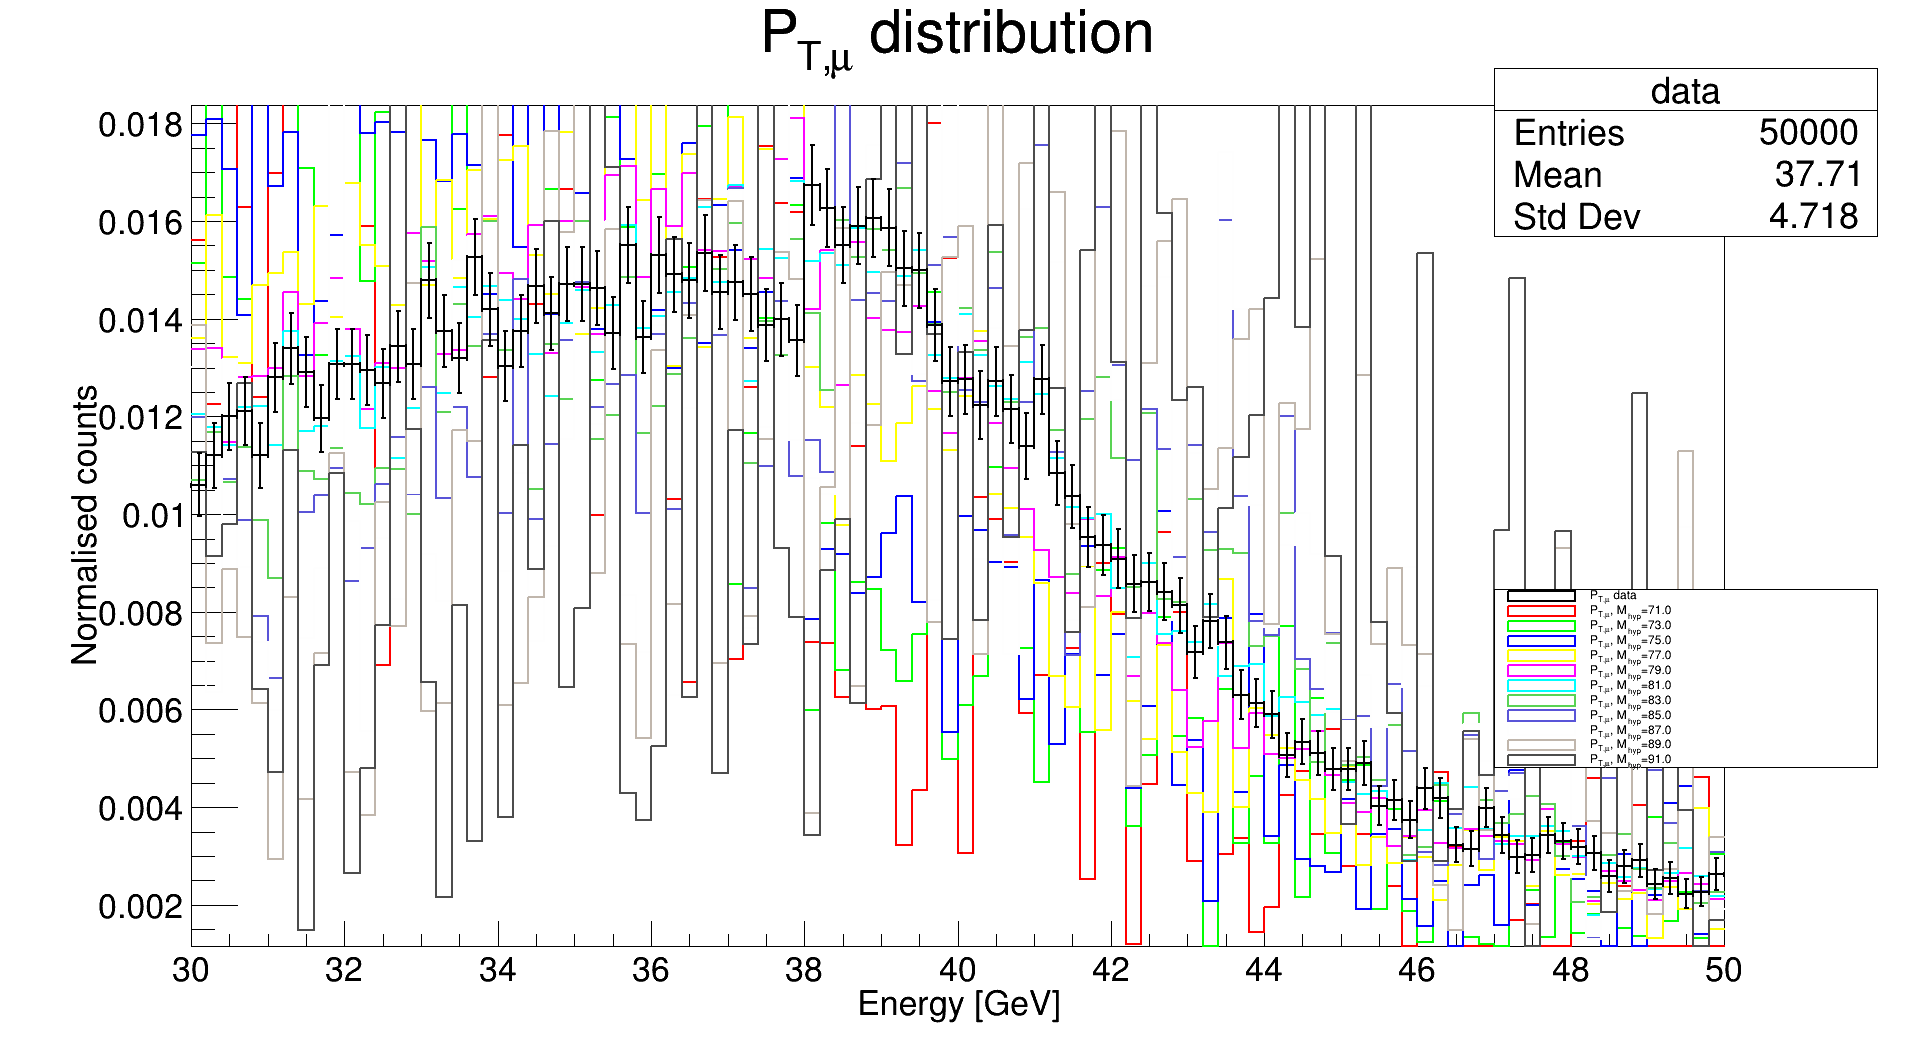
\includegraphics[width=\columnwidth]{/home/physics/phuxdp/Desktop/PX402 Physics Project/WBosonProject/noQED/plots/muPT_80.36010913_2.07041274_between_71_and_91.png}
		\caption{\small Hypothesis masses Number of data points used: 99999,\\
mean expected W mass: 80.36010913 $[GeV/c^{2}]$,\\
mean hypothesis masses $[GeV/c^{2}]$: [<generator object <genexpr> at 0x7f820a339510>],\\
mass width: 2.07041274 $[GeV/c^{2}]$,\\
chi_square value of hypothesis fit: 112.07408778430181. }
		\label{fig: fig_0}
	\end{figure}
    Notes: \\
    1) Using mu\_born\_PT as pseudodata and  Mu\_Pt as model/hypothesis\\
    2) Using full run mode\\
       \begin{figure}[tb]
		\centering
		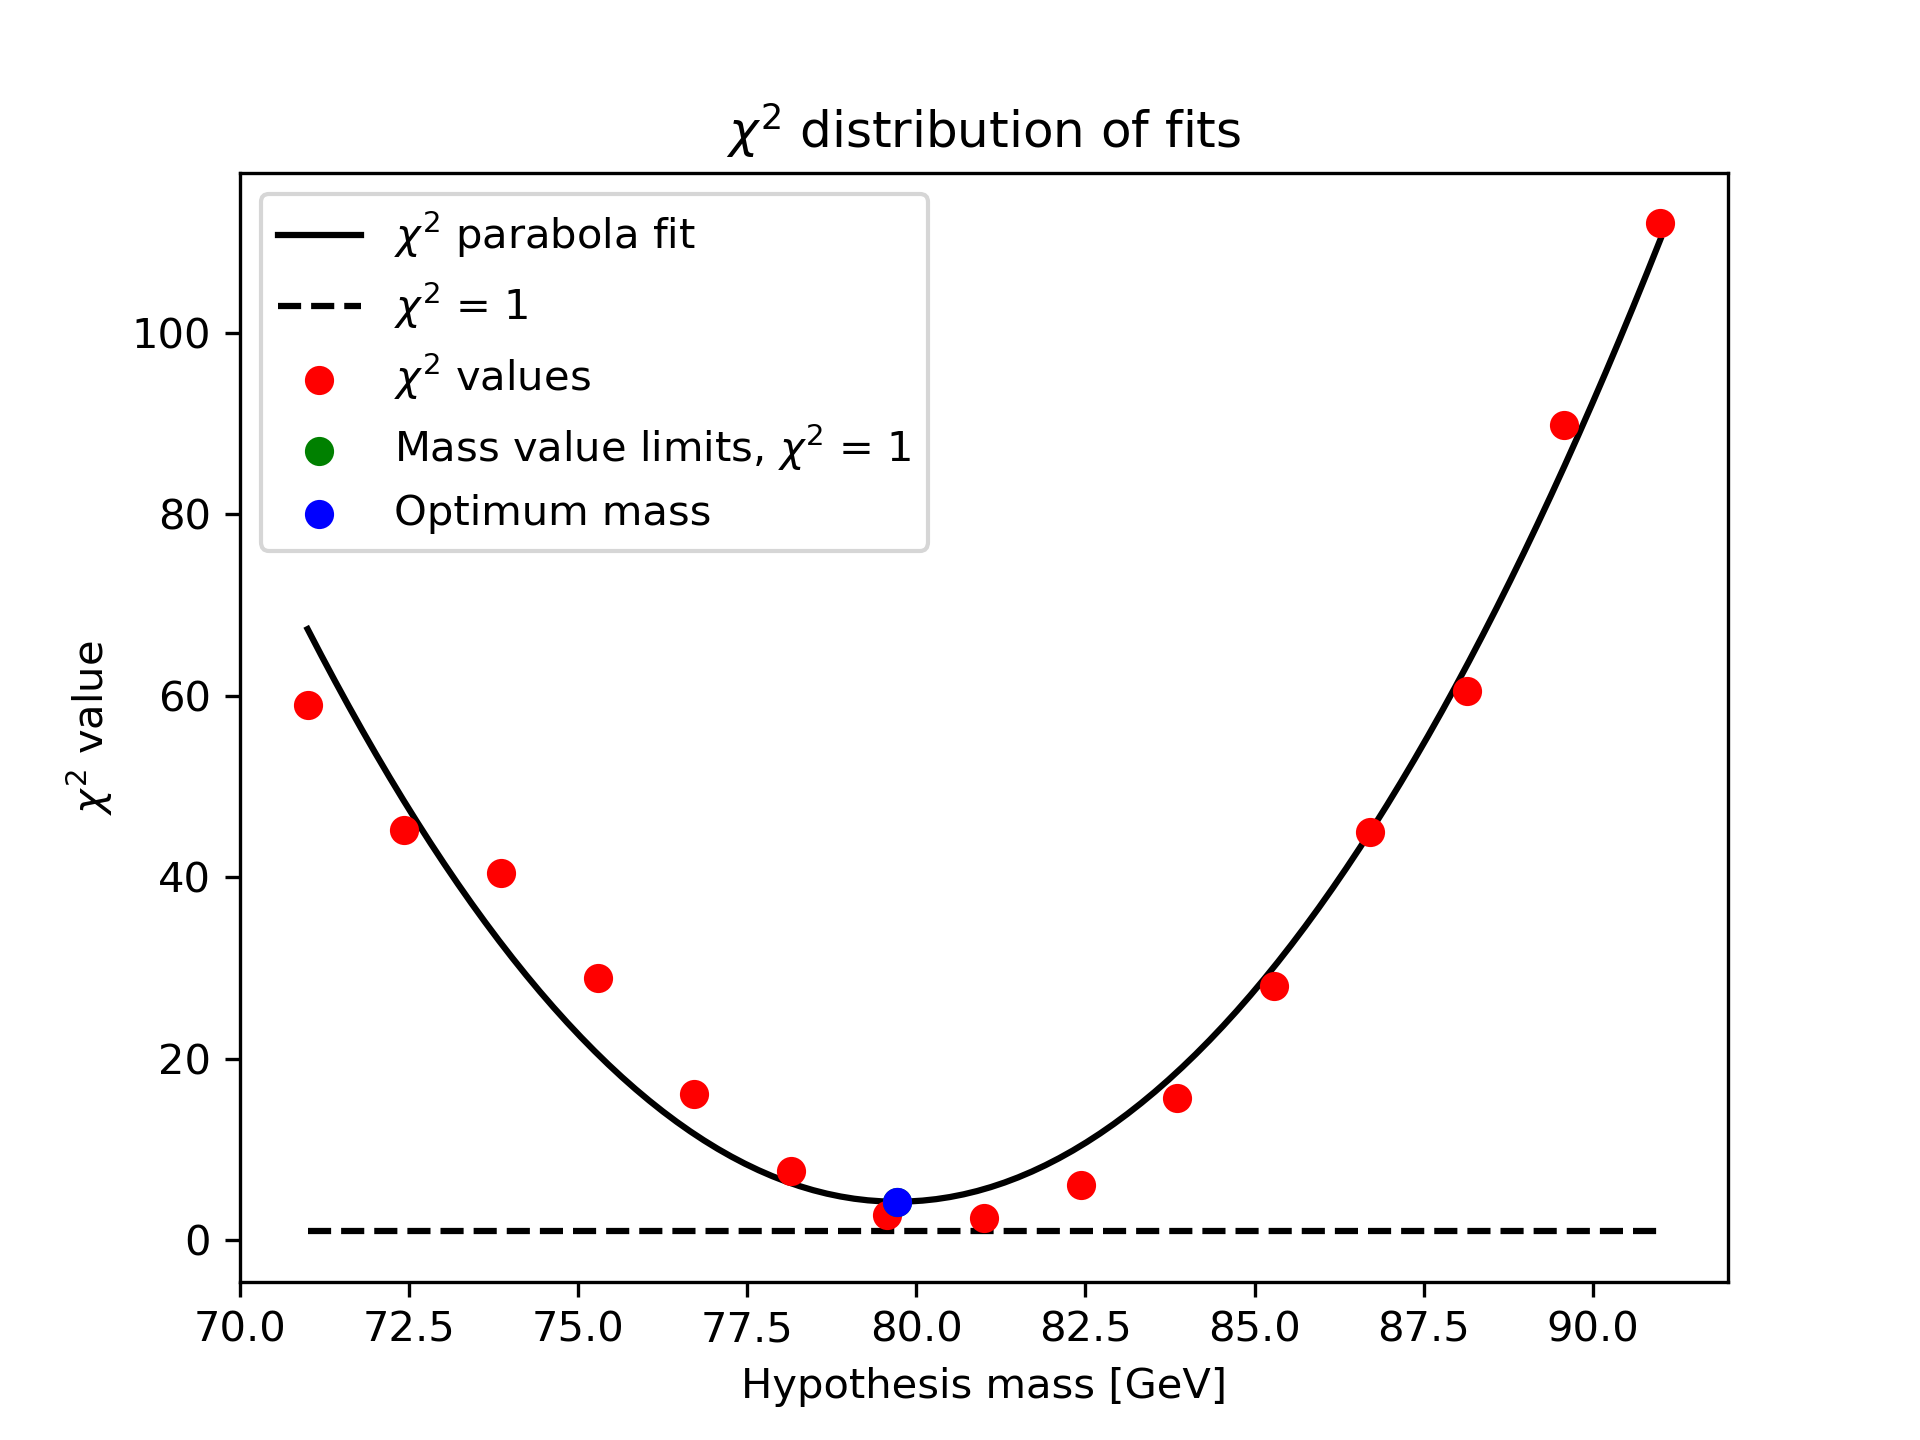
\includegraphics[width=\columnwidth]{/home/physics/phuxdp/Desktop/PX402 Physics Project/WBosonProject/noQED/plots/chi_square_fits_muPT_80.36010913_2.07041274_between_71_and_91.png}
		\caption{\small $\chi^2$ of hypothesis masses. }
		\label{fig: fig_chi_square}
	\end{figure}

    \begin{figure}[tb]
		\centering
		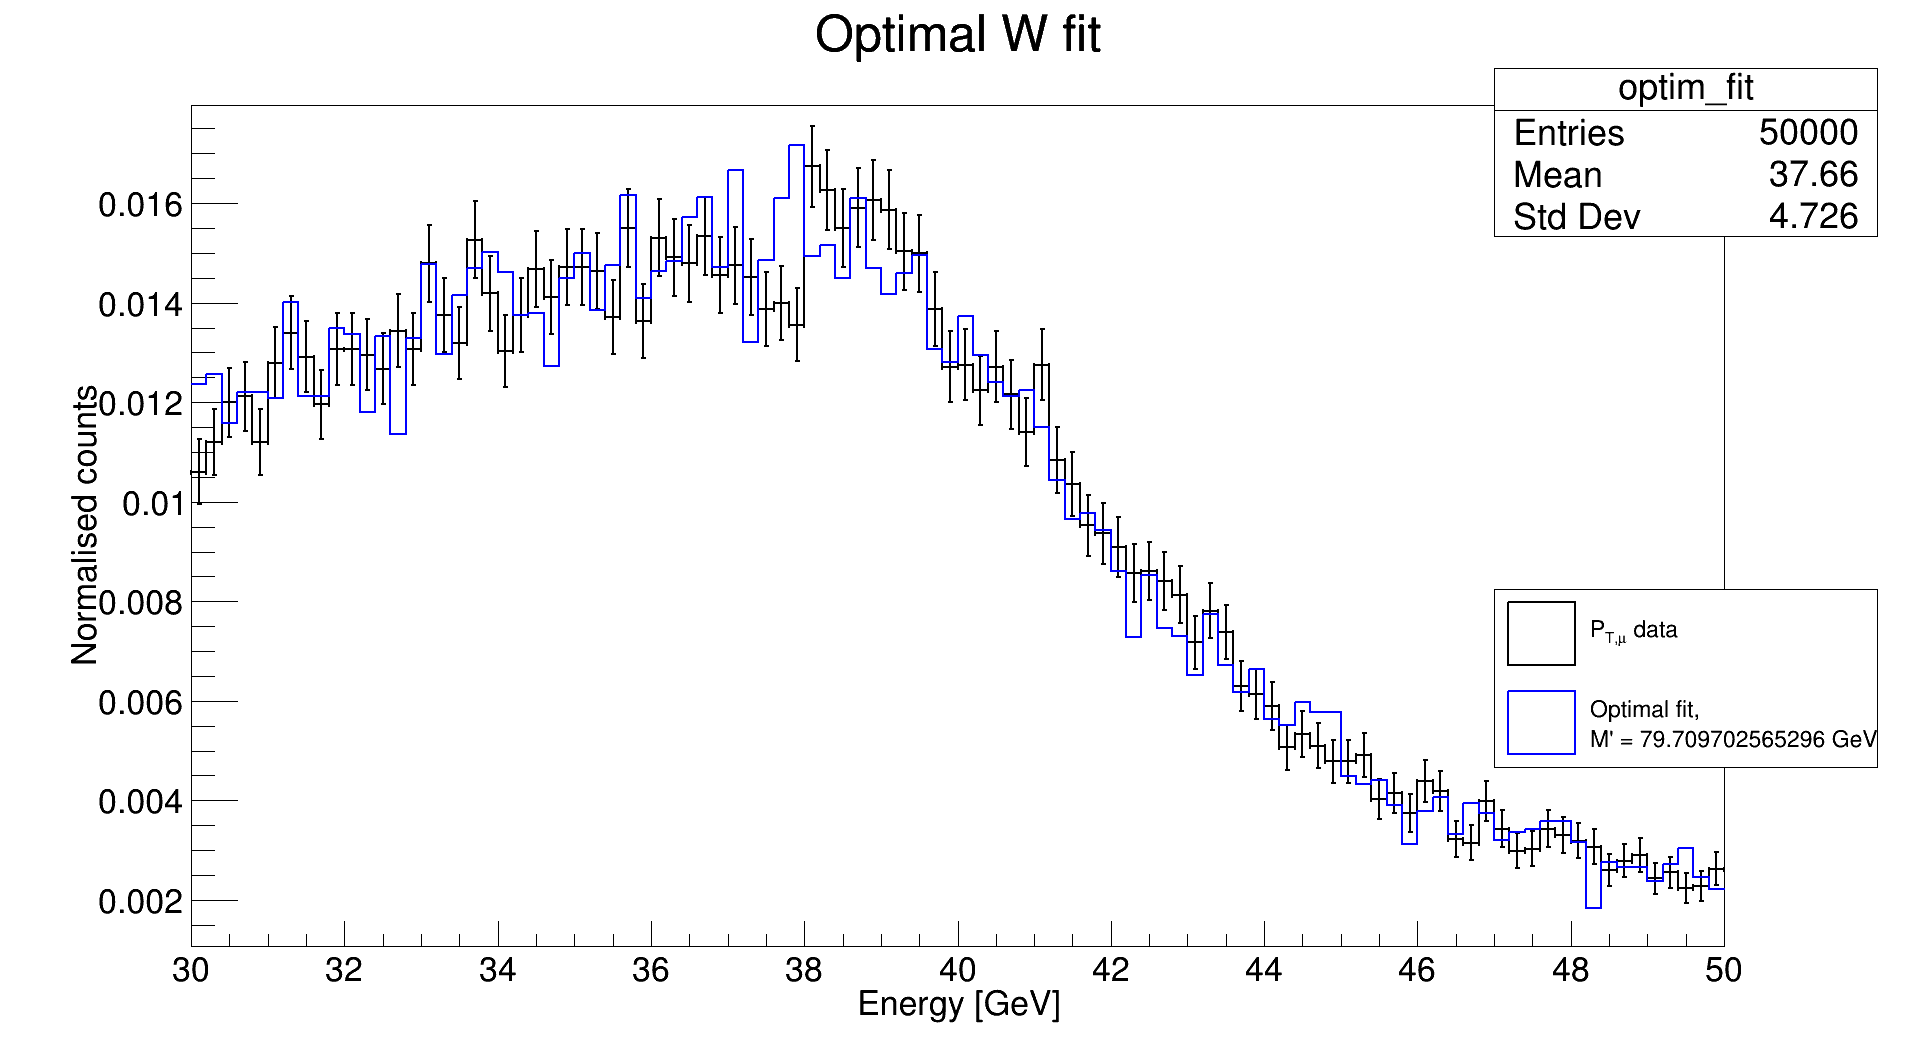
\includegraphics[width=\columnwidth]{/home/physics/phuxdp/Desktop/PX402 Physics Project/WBosonProject/noQED/plots/optimum_muPT_80.36010913_2.07041274_between_71_and_91.png}
		\caption{\small Data and optimum fit with $\chi^2 = 1.8980230486966845$. Used the hypothesis mass of 79.65868412035844 $[GeV/c^{2}]$. }
		\label{fig: fig_optim_parms}
	\end{figure}
    
\end{document}